\section{Architecture}

\begin{figure}[t]
    \centerline{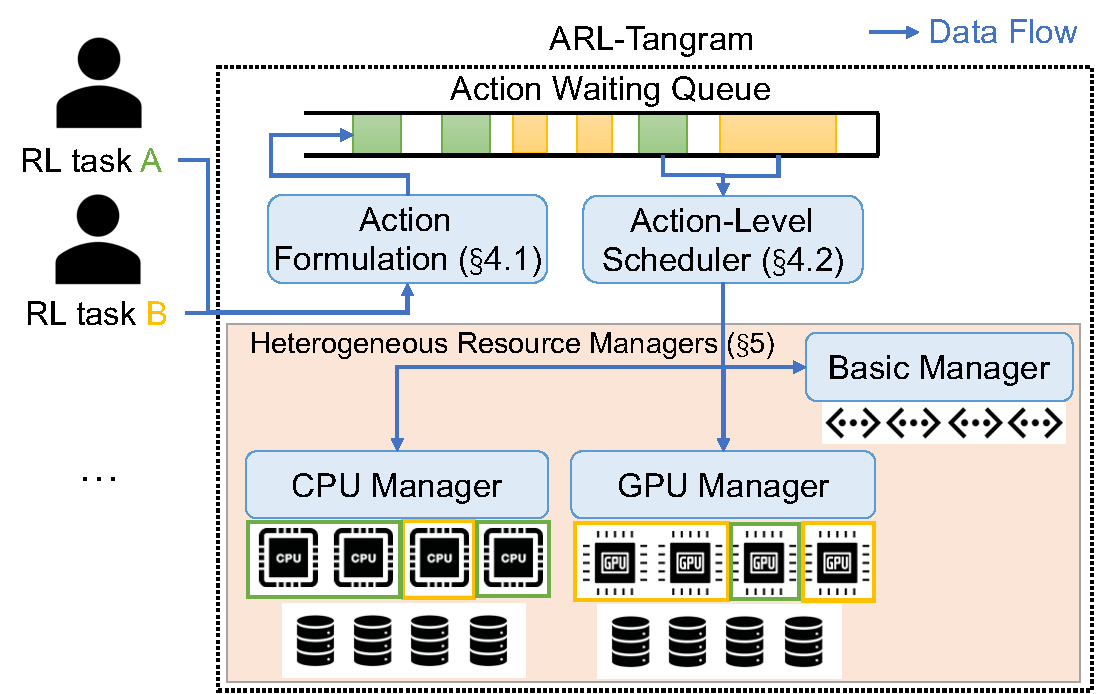
\includegraphics[width=0.6\linewidth]{figures/arch.pdf}}
    \vspace{-0.1in}
    \caption{System overview of \sysname.}
    \label{fig:arch_arch}
    \vspace{-0.15in}
\end{figure}

To address the multifaceted over-provisioning issues inherent in current agentic RL training—within trajectories, and within RL tasks. 
We propose a unified action-level platform, \sysname. 
Our architecture decouples external resource management from the primary RL training cluster, shifting the granularity of control from long-lived trajectories to individual atomic interactions, or actions.

As shown in Figure~\ref{fig:arch_arch}, the system serves as a centralized intermediary between diverse RL Tasks and heterogeneous external resources. 
The workflow follows a standardized execution cycle:
(1) Action Submission: During the rollout phase, when an agentic LLM invokes a tool, or reward calculation with external resources, it submits a request to \sysname.
(2) Unified Formulation \& Queuing: Through formulation, \sysname translates various external resource invocations into unified actions. Hence, these requests are submitted to a Unified Action Queue.
(3) Elastic Scheduling: The scheduler schedules the actions in the waiting queue under the constraints of external resources, and coordinates with specialized Resource Managers (e.g., CPU, GPU, API) to elastically allocate the resources based on real-time system state and action formulation.
(4) Action Execution: After the units of resources are decided, actions are independently executed on the resources allocated by heterogeneous resource managers.
(5) Transmit \& Observation: Once an execution is complete, the results are transmitted back to the RL framework, allowing it to proceed with the next LLM generation.

There are three main components in \sysname---the action formulation module(\S\ref{sec:design_modeling}), the action-level scheduler(\S\ref{sec:design_scheduling}), and heterogeneous resource managers(\S\ref{sec:design_resource_managing}).
The foundation of our architecture treats every atomic invocation as an action.
Thus, the formulation module models the costs and performance elasticity of various actions in a unified way.
Then, the scheduler decides whether an action is able to schedule under the resource constraints, and allocates resources elastically to minimize the action completion time (ACT).
In this way, \sysname reduces the time LLMs spend waiting for external resource invocations, further accelerating the RL training.
With scheduling decisions, heterogeneous resource managers are responsible for efficient resource allocation and sharing.
Using a unified resource interface, our resource managers, including Basic Manager, CPU Manager and GPU Manager, employ domain-specific techniques to improve system robustness, resource utilization, and action speed.
